% !TEX root = cha-application.tex
\documentclass[../../main.tex]{subfiles}

\begin{document}

\section{Class Hierarchy: Wassis vs. PlantUML}

\label{sec:wassis_vs_plantuml}

To evaluate \wassis, we visualize the complete inheritance hierarchy of the \texttt{Magnitude} class in Pharo 13. The hierarchy contains 41 classes at different levels. We compare the result produced by \wassis with the diagram generated by \plantuml~\citeonline{plantuml}, as shown in \figref{fig:magnitude_comparison}. Specifically, \figref{fig:magnitude_plantuml} displays the traditional layout produced by \plantuml, while \figref{fig:magnitude_wassis} shows the output generated by \wassis.

% \begin{figure}[htbp]
%     \centering
%     \includegraphics[width=\textwidth]{figures/application/magnitude_hierarchy.pdf}
%     \caption{\wassis full hierarchy for the \texttt{Magnitude} class.}
%     \label{fig:magnitude_wassis}
% \end{figure}

% \begin{figure}[p]
%     \centering
%     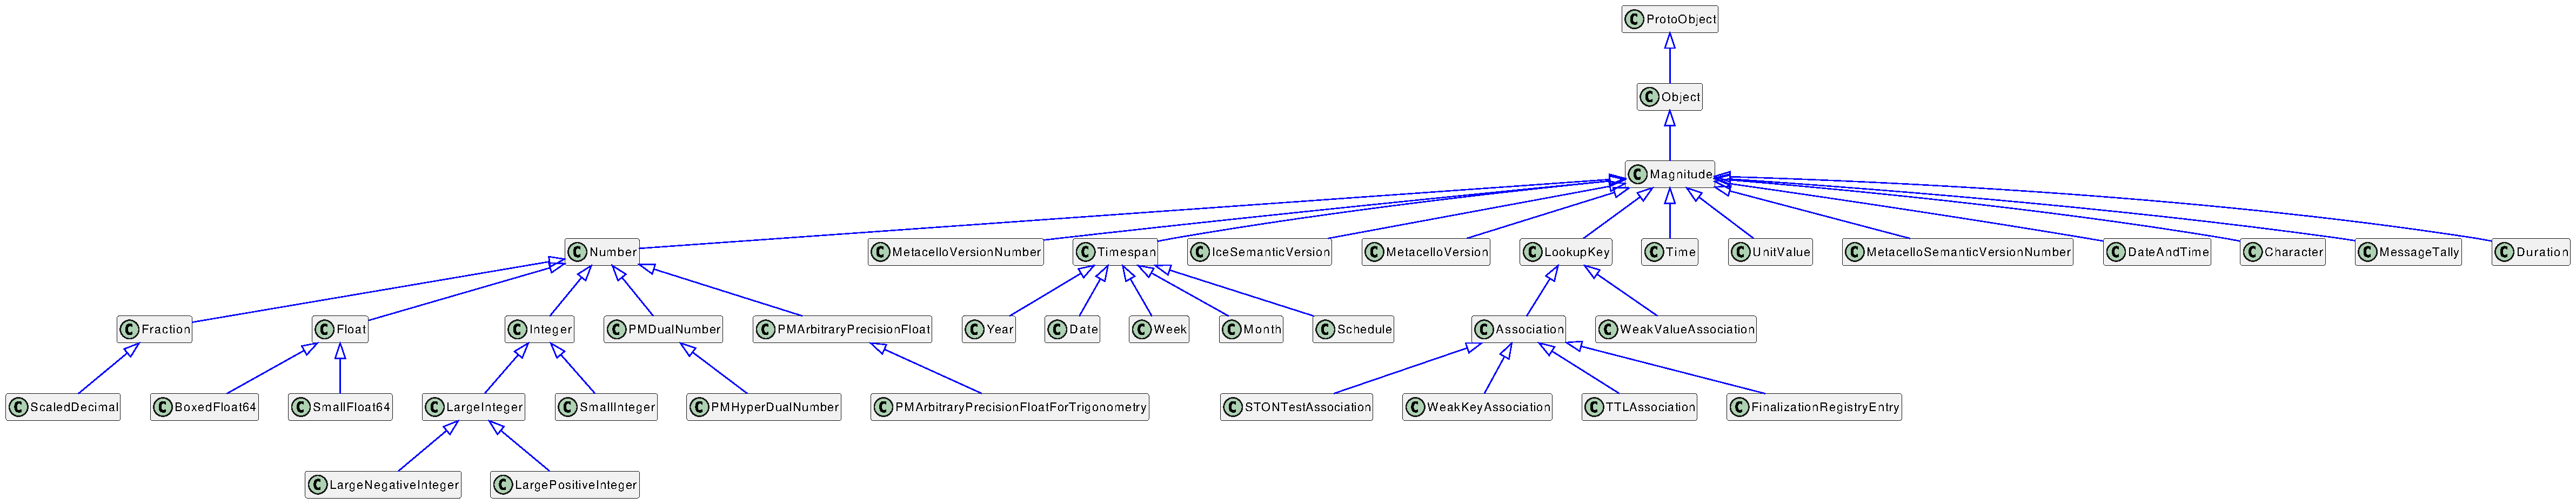
\includegraphics[height=0.24\textheight, angle=90]{figures/application/magnitude_plantUML.pdf}
%     \caption{PlantUML full hierarchy for the \texttt{Magnitude} class.}
%     \label{fig:magnitude_plantuml}
% \end{figure}

\begin{figure}[htbp]
    \centering
    \begin{subfigure}[c]{0.40\textwidth}
        \centering
        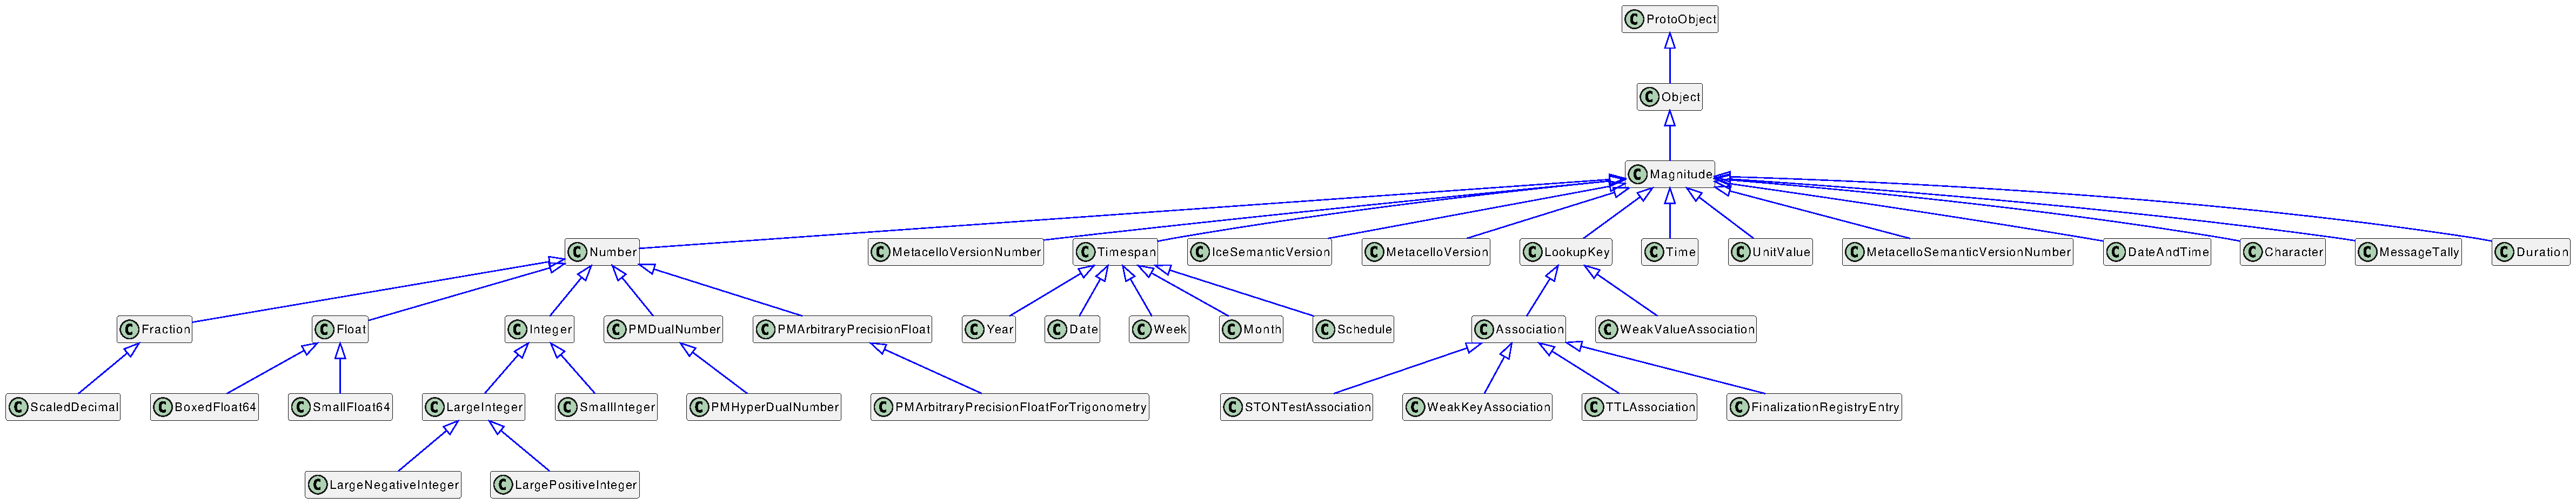
\includegraphics[height=0.183\textheight, keepaspectratio, angle=90]{figures/application/magnitude_plantUML.pdf}
        \caption{\plantuml \texttt{Magnitude} hierarchy.}
        \label{fig:magnitude_plantuml}
    \end{subfigure}
    \hfill
    \begin{subfigure}[c]{0.58\textwidth}
        \centering
        \includegraphics[width=\textwidth, keepaspectratio, angle=90]{figures/application/magnitude_hierarchy}
        \caption{\wassis \texttt{Magnitude} hierarchy.}
        \label{fig:magnitude_wassis}
    \end{subfigure}
    \caption{Comparison for the \texttt{Magnitude} class between \plantuml (a) and \wassis (b).}
    \label{fig:magnitude_comparison}
\end{figure}

\subsection{Layout}

The two tools organize the hierarchy in different ways. \wassis produces a compact two-dimensional layout, where classes can be placed in all directions. The root class, \texttt{Magnitude}, is placed at the center, while the other classes are distributed around it, creating a star structure. The use of MDS keeps related classes close to each other, while the grid allows the hierarchy to use the available space in all directions.

This layout makes the complete hierarchy fit in a relatively small area, making it possible to see the whole structure at a glance.

\plantuml uses a hierarchical layout, where classes are organized into horizontal levels. Classes at the same hierarchy depth are placed on the same level, so the hierarchy grows from top to bottom and in width.

In this example, the large number of subclasses of \texttt{Magnitude} makes the first level very wide. If the diagram was kept in its original orientation, it would need to be scaled to fit the available width, making it difficult to read. It is therefore rotated by 90 degrees in \figref{fig:magnitude_plantuml}. For larger hierarchies, horizontal scrolling is required to inspect the complete diagram. As a result, the complete structure cannot be viewed at once without scrolling, unlike in \wassis, where the compact layout allows the whole hierarchy to be seen at a glance.

\plantuml nevertheless has an important advantage: classes at the same hierarchy depth are placed on the same level. This makes the depth of the hierarchy immediately visible and makes it easy to follow the structure from one level to the next. In \wassis, classes are positioned according to the structure of the graph rather than their hierarchy depth. Therefore, classes at the same hierarchy level are not necessarily placed at the same distance from the root, making this information less direct.

\subsection{Path Representation}

The two visualizations also differ in how relationships between classes are represented. \wassis uses path merging to combine paths that have the same target, reducing the number of paths and keeping the visualization cleaner.

In the shown example, the paths generated by \wassis do not overlap. This makes the relationships easier to follow, even in areas with many connections. Path merging is most useful when several relationships share the same target, as it avoids drawing redundant path segments.

\plantuml, on the other hand, generates a separate arrow for each relationship. When several relationships connect to the same class, the arrows can overlap or become very close to each other. In the shown example, several arrows overlap, making it difficult to follow them individually.

Path merging therefore helps \wassis keep the visualization clean. In \plantuml, representing each relationship with a separate arrow makes all connections explicit, but can also lead to visual clutter when many relationships are present.

\subsection{Class Identification}

A clear advantage of \plantuml is that class names are displayed in the diagram, allowing the user to identify a class directly.

In contrast, \wassis intentionally omits class names on the main canvas to prevent text label collisions. Class information can instead be accessed on demand through interactive features such as hover tooltips.

This is an important trade-off. \plantuml provides more textual information directly on the canvas, while \wassis gives more space to the visual structure of the system and maintains readability at scale.

\subsection{Execution Time}

The main limitation observed in this example is execution time. Generating the \wassis visualization shown in \figref{fig:magnitude_wassis} required approximately two weeks of computation. This is mainly because WFC has to find a valid arrangement of all paths.

\plantuml, in contrast, generates the corresponding diagram in a much shorter time. This makes \plantuml more suitable when a diagram has to be generated quickly.

The execution time of \wassis is therefore an important limitation for larger software systems. This cost should be considered when choosing \wassis for practical use, especially when the visualization needs to be regenerated frequently.

% \subsection{Summary}

% The comparison highlights the trade-offs between the two visual tools. \wassis offers a compact layout with clear, non-overlapping paths, making the overall structure fit into a small view. However, it requires more interaction to identify classes and takes significantly more time to compute. PlantUML provides explicit class names and clear hierarchy levels, but its diagrams can become very wide and contain overlapping arrows when many subclasses are present.

The main differences between \wassis and \plantuml are summarized in Table~\ref{tab:wassis_plantuml_comparison}.

\begin{table}[ht]
    \centering
    \begin{tabular}{p{0.18\textwidth} p{0.35\textwidth} p{0.35\textwidth}}
        \textbf{} & \textbf{Wassis} & \textbf{PlantUML} \\ \hline
        \textbf{Layout} & Compact star layout; root near the center. & Traditional hierarchical layout. \\
        \textbf{Space} & Uses the space in multiple directions. & Can become very wide for hierarchies with many subclasses. \\
        \textbf{Paths} & Paths remain separated and easier to follow. & Several arrows can become close or overlap. \\
        \textbf{Hierarchy} & Less explicit because classes are positioned according to graph distances. & More explicit because classes are organized by hierarchy level. \\
        \textbf{Class Names} & Not shown directly on the main visualization. & Shown directly on each class. \\
        \textbf{Time} & High for this example; approximately two weeks. & Milliseconds. \\ \hline
    \end{tabular}
    \caption{Comparison between \wassis and \plantuml for the \texttt{Magnitude} hierarchy.}
    \label{tab:wassis_plantuml_comparison}
\end{table}

\end{document}